

\begin{comment}
    \begin{figure*}[t]
      \centering
      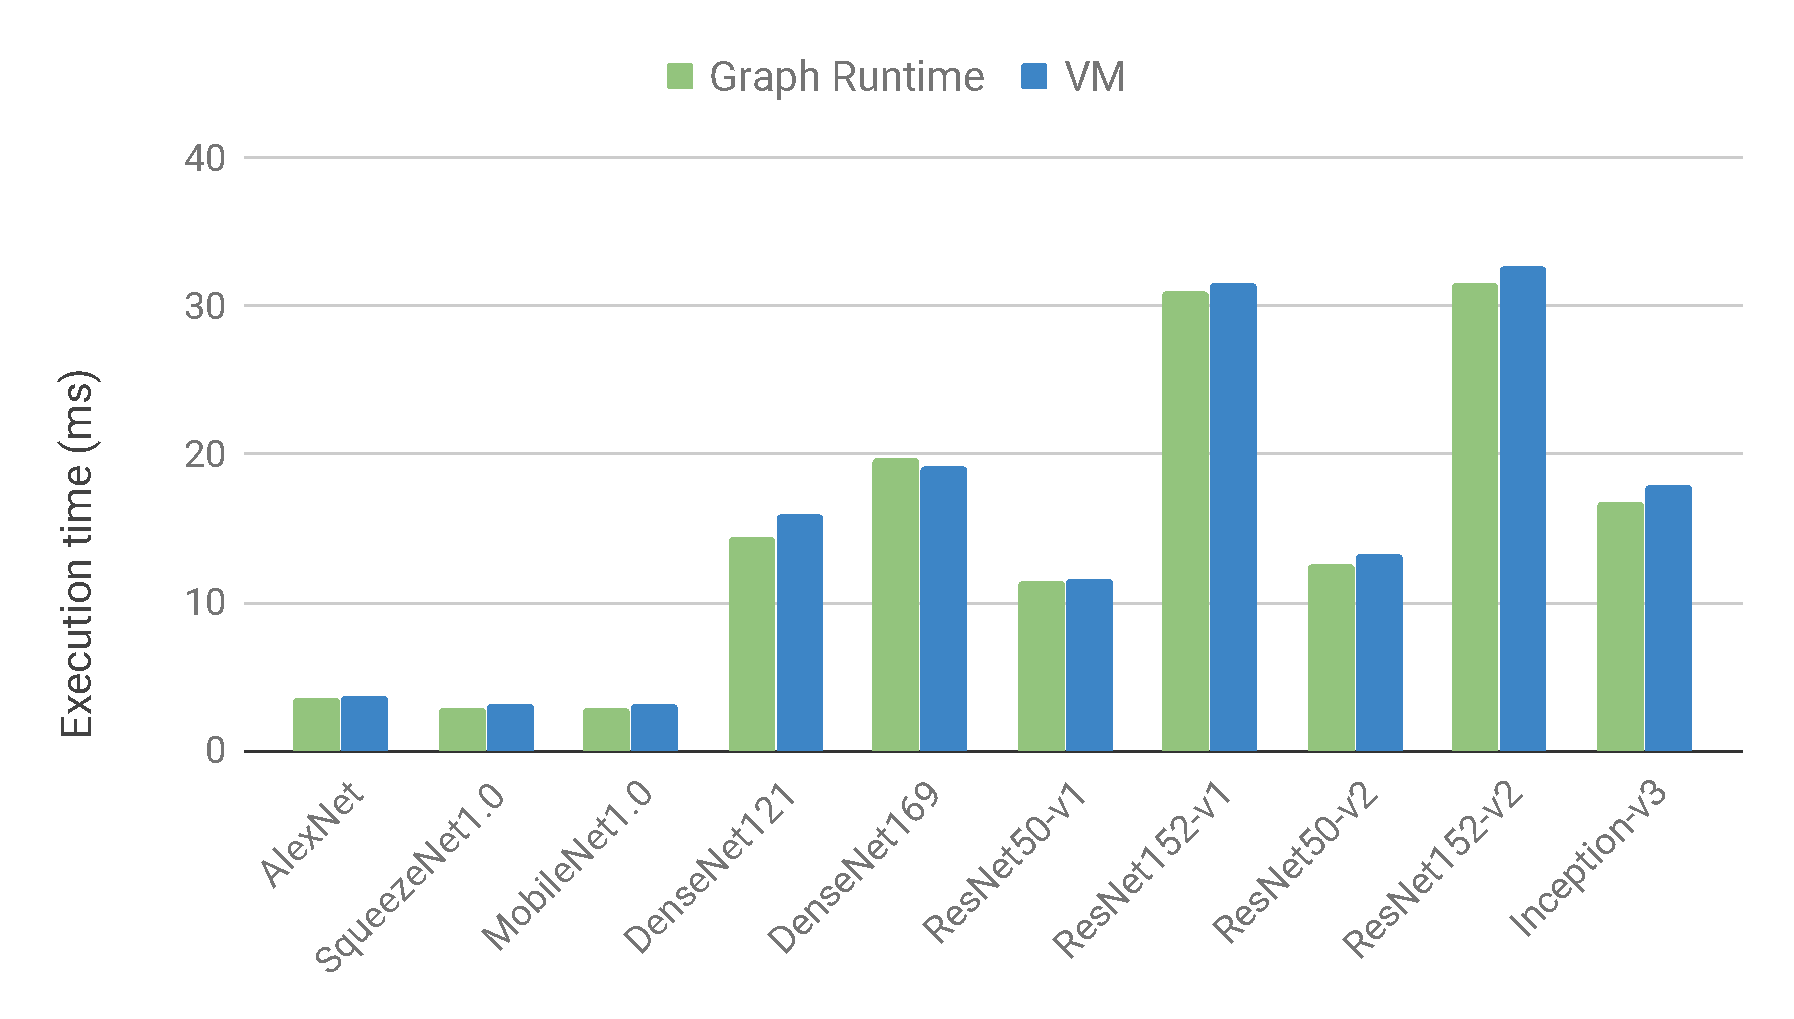
\includegraphics[width=.8\linewidth]{figs/cv_models.pdf}
      \caption{Benchmarking results of graph runtime vs. Relay.}
      \label{fig:benchmark}
    \end{figure*}

    \begin{table*}[t]
    \centering
    \begin{tabular}{llllrrc}
    \toprule
    \multicolumn{1}{c}{\multirow{2}{*}{input size}} & \multicolumn{1}{c}{\multirow{2}{*}{hidden size}} & \multicolumn{1}{c}{\multirow{2}{*}{\# layers}} & \multicolumn{1}{c}{\multirow{2}{*}{seq length}} & \multicolumn{2}{c}{latency (ms)}                         & \multicolumn{1}{c}{\multirow{2}{*}{speedup ($\times$)}} \\
    \multicolumn{1}{c}{}                            & \multicolumn{1}{c}{}                             & \multicolumn{1}{c}{}                          & \multicolumn{1}{c}{}                            & \multicolumn{1}{c}{MxNet} & \multicolumn{1}{c}{Relay VM} & \multicolumn{1}{c}{}                             \\
    \midrule
    100                                             & 100                                              & 1                                             & 1                                               & 0.53                      & 0.03                         & 18.4                                             \\
    100                                             & 100                                              & 1                                             & 20                                              & 4.74                      & 0.52                         & 9.2                                              \\
    100                                             & 100                                              & 1                                             & 100                                             & 21.75                     & 2.57                        & 8.5                                              \\
    100                                             & 100                                              & 2                                             & 100                                             & 30.53                     & 4.79                         & 6.4                                              \\
    100                                             & 100                                              & 3                                             & 100                                             & 55.47                     & 7.04                         & 7.9                                              \\
    200                                             & 600                                              & 3                                             & 100                                             & 67.14                     & 35.16                        & 1.9                                              \\
    400                                             & 1150                                             & 3                                             & 100                                             & 166.54                    & 123.54                       & 1.3                                              \\
    1500                                            & 1500                                             & 2                                             & 100                                             & 182.71                    & 138.78                       & 1.3
    \\\bottomrule
    \end{tabular}

    \caption{Compare performance of LSTM models between MxNet and Relay VM.}
    \label{tab:lstm}
    \end{table*}

    We evaluated the model inference with the VM against the TVM graph runtime on a number of popular vision models, including AlexNet, ResNet, MobileNet, VGG, DenseNet, SqueezeNet and Inception. Models are from GluonCV model zoo.  We repeated the inference 100 times for each model, obtained the performance result by averaging the execution times. All experiments were performed on Amazon EC2 C5.9xlarge instance (Intel Skylake-SP, 72 GiB memory, 18 physical cores, featured with AVX-512). In general, VM reached comparable inference performance even some optimizations were not plugged. As shown in \autoref{fig:benchmark}, we observed VM provided 2.59\% performance improvement on DenseNet169. On the rest of models, VM introduced some performance regression. We saw 11.3\% performance drop on SqueezeNet1.0.

    We also evaluated the inference performance of recurrent models, which requires control flow support. We choose LSTM model \citep{hochreiter1997long} and vary the input size, hidden size, number of layers, and sequence length. We measured the execution time of LSTM models for both MxNet MKL 1.4.1 and Relay VM on Amazon EC2 C5.9xlarge instance. \autoref{tab:lstm} shows that Relay VM can achieve 6.4-18.4$\times$ speedup on small LSTM models and 1.3-1.9$\times$ speedup on larger models.
    \end{comment}

    \section{Evaluation}
    \label{sec:eval}

    This section evaluates the performance of Relay on dynamic models against existing state-of-the-art solutions, as well as discussing the role of the optimizations performed by Relay. Specifically, the section seeks to answer the following questions:
    \begin{enumerate}
        \item What is the overall performance of Relay for dynamic models when compared against state-of-the-art alternatives on various hardware platforms?
        %\item How much overhead does Relay introduce for static models on top of the state-of-the-art solutions?
        \item How much overhead does Relay VM introduce for handling dynamism at runtime?
        \item How effective are the proposed optimization techniques, such as memory planning and symbolic codegen?
    \end{enumerate}

    %\yida{Evaluate the execution time of the bytecode as a portion of the total execution time, to show that VM overhead is negligible}
    %\note{End-to-end: BERT, LSTM, Tree-LSTM on Intel CPU, ARM CPU, NVidia GPU; Relay-runtime vs. graph runtime. Optimization implication: Kernel dispatch or not; memory planning or not; number of dispatched kernels.}
    \subsection{Experiment setup}
    \label{sec:eval:setup}

    All experiments were conducted on Amazon EC2 instances. We evaluated Relay on three hardware platforms: Intel Skylake CPUs (c5.9xlarge, 18 physical cores, hereinafter called {\em Intel CPU}), Nvidia Tesla T4 GPUs (g4dn.4xlarge, 1 card, 2,560 CUDA cores, hereinafter called {\em Nvidia GPU}), and ARM Cortex A72 (a1.4xlarge, 16 physical cores, hereinafter called {\em ARM CPU}). Although all tests are done on the cloud, our results of ARM CPU are portable to the edge devices, e.g. Raspberry Pi, due to the same architecture. %All cores have uniform memory access.

    To study the efficiency of Relay in handling dynamic models, we compared it with mainstream deep learning frameworks, including TensorFlow (v1.15), MXNet (v1.6), PyTorch (v1.5) \footnotemark, as well as dynamic-specific systems TensorFlow Fold based on TensorFlow v1.0.
    \footnotetext{We use PyTorch v1.4 on ARM CPU because PyTorch v1.5 fails to build on ARM instance.}
    %For TensorFlow Fold, its execution latency would include the compilation time (\zhicomment{@haichen, we probably need a bit argument here for why compile time is included.}).
    We were unable to compare Relay with Cavs~\citep{xu2018cavs}, JANUS~\citep{jeong2019janus}, or Jeong et al.\citep{jeong2018improving} as none of them is open-source. No public deep learning compiler has claimed support for dynamic models.
    %For static models, TVM~\citep{tvm_osdi18} was selected as the baseline to investigate the cost of Relay since it represents the state-of-the-art performance for static models on CPUs~\citep{liu2019optimizing}.

    Three popular models that represent different classes of dynamism were chosen in this experiment, viz. LSTM~\citep{lstm} (dynamic control flow), Tree-LSTM~\citep{tree_lstm} (dynamic data structure), and BERT~\citep{devlin2018bert} (dynamic data shape).
    The input size / hidden size used in the LSTM and Tree-LSTM model are 300/512 and 300/150, respectively.
    %while we use input size 300 and hidden size 150 in the Tree-LSTM model.
    We used BERT base implementation.
    For LSTM and BERT, we used Microsoft Research's Paraphrase Corpus (MRPC)~\citep{dolan2005microsoft} with variable input lengths as our input dataset. For Tree-LSTM, we used the Stanford Sentiment Treebank (SST)~\citep{socher2013recursive} with various tree structures as the input dataset.
    %\note{missing model size, e.g. LSTM number of layers, length, BERT size}
    %For the measurement of the overhead on static models, we completed model inference for ResNet~\citep{he2016deep}, MobileNet~\citep{howard2017mobilenets}, VGG~\citep{simonyan2014very}, and SqueezeNet~\citep{iandola2016squeezenet} on the ImageNet dataset~\citep{deng2009imagenet}. Only one input is needed to feed to the system each time for the task of model inference.

    \subsection{Overall performance}
    \label{sec:eval:overall}
    We compare the overall performance of Relay against baselines for each dynamic models. Relay successfully accomplished inference for all models on all platforms. However, not all baseline systems could perform inference for these models. For instance, TensorFlow Fold was not designed to process LSTM and BERT hence no result was obtainable, and Tree-LSTM only runs on PyTorch and TensorFlow Fold as other frameworks cannot handle dynamic data structures. Finally the model inference of Tree-LSTM on Nvidia GPU was omitted as it's hard to saturate GPU compute capability due to too many control flows and its model size, making GPUs less favorable deployment targets.
    % typical use cases.

    The baseline systems all make use of third-party kernel libraries to achieve high-performance by leveraging the heavily hand-optimized operators. We observe that dynamic models are often well-optimized on a single platform but perform poorly in other frameworks or on other targets. However, Relay has the ability to select either the self-compiled kernels or the ones provided by third-party library based on which one maximizes performance. It uses dynamic dispatch logic to invoke the selected kernels using platform-independent bytecode at runtime. This enables Relay to deliver portable and consistent results as many compiler optimizations are platform agnostic.
    %, and Relay has the freedom to choose whatever implementation that produces better performance.

    First, the latency results of Relay, MXNet, PyTorch, and TensorFlow on LSTM are shown in \autoref{tab:lstm}. Relay consistently outperforms the baseline on both 1- and 2-layer cases. For example, it reduces the latency of 1-layer LSTM model inference by $\fpeval{round(79.3 / 47.8, 1)}\times$, $\fpeval{round(212.9 / 47.8, 1)}\times$, and $\fpeval{round(301.4 / 47.8, 1)}\times$ over PyTorch, MXNet, and TensorFlow on Intel CPU,
    and $\fpeval{round(110.3/93.0, 1)}\times$, $\fpeval{round(135.7/93.0, 1)}\times$, $\fpeval{round(304.7/93.0, 1)}\times$ on Nvidia GPU, respectively.
    %On Nvidia GPU, Relay reduces the latency by  over PyTorch, MXNet, and TensorFlow on Nvidia GPU, respectively.
    On ARM CPU, Relay decreases the latency numbers even more remarkably, i.e. $\fpeval{round(1729.5 / 182.2, 1)}\times$ over PyTorch, $\fpeval{round(3695.9 / 182.2, 1)}\times$ over MXNet, and $\fpeval{round(978.3 / 182.2, 1)}\times$ over TensorFlow, respectively.
    The similar trend applies to 2-layer case of the LSTM model.
    We observe that latency on Nvidia GPU is higher than Intel CPU. This is because the size of LSTM model is relative small so that it cannot fully utilize the massive parallelism in the GPU.
    The significant performance improvement is due to Relay encoding the control flow into platform-independent instructions that have minimal overhead while deep learning frameworks use control flow specific primitives to process the sequence, which introduces a large performance penalty.

    \begin{table}[t]
    \centering
    \small
    \begin{tabular}{p{0.9cm}|ccc|ccc}
    \toprule
    Unit: & \multicolumn{3}{c|}{1 layer} & \multicolumn{3}{c}{2 layers} \\
    $\mu$s/token & Intel & NV & ARM & Intel & NV & ARM \\ \midrule
    Relay & \bf{47.8} & \bf{93.0} & \bf{182.2} & \bf{97.2} & \bf{150.9} & \bf{686.4} \\
    PT & 79.3 & 110.3 & 1729.5 & 158.1 & 214.6 & 3378.1 \\
    MX  & 212.9 & 135.7 & 3695.9 & 401.7 & 223.8 & 7768.0 \\
    TF & 301.4 & 304.7 & 978.3 & 687.3 & 406.9 & 2192.8 \\
    \bottomrule
    \end{tabular}
    \caption{LSTM model inference latency of Relay, PyTorch (PT), MXNet (MX), and TensorFlow (TF) on Intel CPU, Nvidia (NV) GPU, and ARM CPU.}
    \label{tab:lstm}
    \end{table}

    Next, we inspect the performance of model inference on Tree-LSTM as exhibited in \autoref{tab:treelstm} by comparing Relay with PyTorch and TensorFlow Fold. The table shows that Relay runs substantially faster than the baselines. On PyTorch, the performance speedups are $\fpeval{round(701.1/40.3, 1)}\times$ on Intel CPU and $\fpeval{round(1711.1/86.3, 1)}\times$ on ARM CPU as PyTorch uses Python to handle the tree data structure. TensorFlow Fold is $\fpeval{round(209.9/40.3, 1)}\times$ slower than Relay on Intel CPU because it has to re-compile upon every input.

    \begin{table}[t]
    \centering
    \begin{tabular}{l|ll}
    \toprule
    Unit: $\mu$s/token        & Intel     & ARM \\ \midrule
    Relay  & \bf{40.3}  & \bf{86.3}  \\
    PyTorch & 701.6 & 1717.1  \\
    TF Fold & 209.9 & --  \\
    \bottomrule
    \end{tabular}
    \caption{Tree-LSTM model inference latency on Intel CPU and ARM CPU. TensorFlow Fold was not built successfully on ARM CPU.}
    \label{tab:treelstm}
    \end{table}

    Third, \autoref{tab:bert} summarizes the performance of BERT for Relay, MXNet, and TensorFlow. The results indicate that Relay outstrips the baselines for all frameworks on all platforms in the experiment. The reduction in latency compared to the best framework on each platform is $\fpeval{round(455.8/307, 1)}\times$, $\fpeval{round(2995.4/2862.6, 2)}\times$, and $\fpeval{round(125.2/95.2, 1)}\times$ on Intel CPU, ARM CPU, and Nvidia GPU, respectively.
    %Surprisingly, Relay is $\fpeval{round(455.8/307, 1)}\times$ faster than MXNet on Intel CPU even the latter was known to be heavily optimized on this platform~\footnote{\url{https://medium.com/apache-mxnet/optimization-for-bert-inference-performance-on-cpu-3bb2413d376c}}.
    The reasons are two-fold: (a) similar to frameworks, Relay is also able to use the well-tuned third-party libraries on Intel CPU (MKL) and Nvidia GPU (cuDNN). (b) Relay can further enjoy the benefit of powerful operator fusion brought by the deep learning compiler. One can observe that we obtained more speedups on the ARM CPU for PyTorch and MXNet as the third-party libraries performed less favorable. However, Relay is only slightly faster than TensorFlow on the ARM CPU. This is because the dense operators (contributing to more than 90\% of the overall latency in Bert) on the ARM CPU was not well optimized by the underlying compiler. Therefore, the performance of the combination of operators it selected is on par with the ones used by TensorFlow.

    In sum, the evaluation results demonstrate that Relay produces more portable performance for all dynamic models on different platforms. Instead, the performance of frameworks is more platform dependent and varies from model to model.

    \begin{table}[t]
    \centering
    \begin{tabular}{l|lll}
    \toprule
    Unit: $\mu$s/token    & Intel  &   Nvidia       &  ARM     \\ \midrule
    Relay     & \bf{307.0} & \bf{95.2} & \bf{2862.6} \\
    PyTorch & 479.5 & 220.4 & 11851.2 \\
    MXNet      & 455.8 & 152.9 & 8628.0   \\
    TensorFlow & 768.7 & 125.2 & 2995.4 \\
    \bottomrule
    \end{tabular}
    \caption{BERT model inference latency on Intel CPU, Nvidia GPU, and ARM CPU.}
    \label{tab:bert}
    \end{table}

    % \begin{figure}[t]
    %     \centering
    %     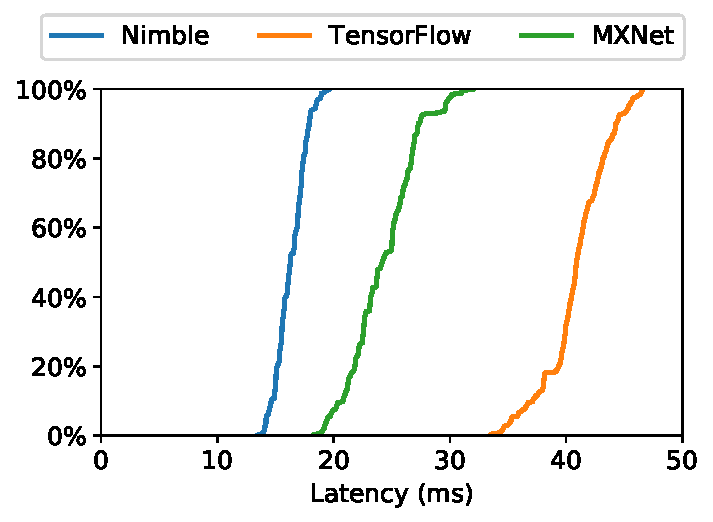
\includegraphics[height=5cm]{figs/bert_cdf_c5.pdf}
    %     \caption{BERT latency CDF on Intel CPU.}
    %     \label{fig:bert-cdf}
    % \end{figure}

    %\subsection{Optimization implications}
    %\label{sec:eval:opt}
    %\subsubsection{Memory planning}

    %\subsubsection{Dynamic kernel dispatch}
    \subsection{Microbenchmark}

    % \begin{table}[t]
    %     \centering
    %     \begin{tabular}{c|cc|cc}
    %         \toprule
    %         \multirow{2}{*}{Device} & TVM & Relay  & kernel & others  \\
    %         & lat. (ms) & lat. (ms) & lat. (ms) &  (ms) \\ %&  (\%) \\
    %         \midrule
    %         Intel  & 19.38 & 24.32 & 21.06 & 3.26 \\% & 13.4\%
    %         ARM & 223.50 & 237.41 & 228.59 & 8.82 \\%& 3.72\% \\
    %         Nvidia & 5.58 & 5.86 & 5.60 & 0.26 \\%& 4.44\% \\
    %         \bottomrule
    %     \end{tabular}
    %     \caption{BERT model latency (sequence length 128) using TVM and Relay on different hardware.
    %     {\it kernel latency} shows the latency of kernel invocation in Relay, and {\it others} shows the extra latency introduced by other instructions.
    %     }
    %     \label{tab:overhead}
    %
    % \end{table}

    % \hide{
    % \begin{figure}[t]
    %     \centering
    %     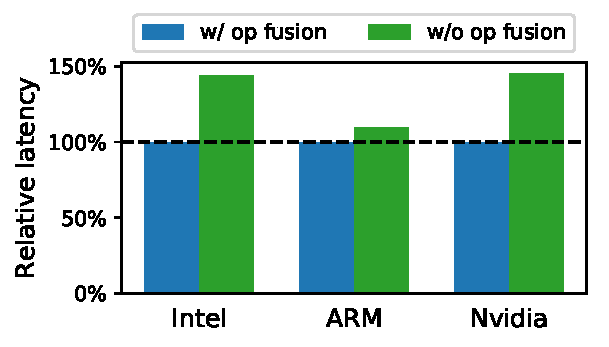
\includegraphics[height=3.5cm]{figs/op_fusion.pdf}
    %     \caption{Relative latency comparison between Relay with and without operator fusion for BERT model with sequence length 128.}
    %     \label{fig:fusion}
    %
    % \end{figure}
    % }

    \begin{figure}[t]
        \centering
        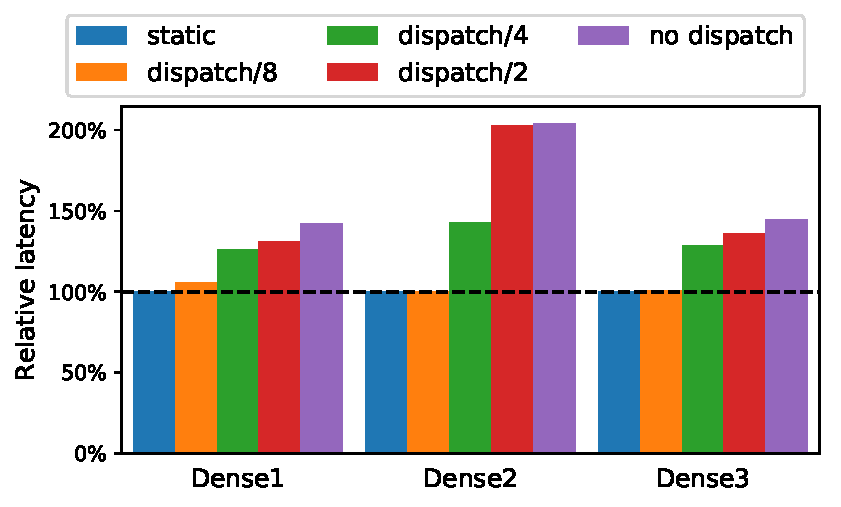
\includegraphics[height=4.5cm]{figs/sym_codegen.pdf}
        \caption{Relative latency comparison between symbolic codegen and static codegen of 3 dense operators on ARM CPU. The latency of kernel compiled with static shapes is used as the baseline. ``dispatch/$k$'' indicates that we generate $k$ symbolic kernels to be dispatched at runtime. ``no dispatch'' means that only one symbolic kernel is generated and therefore no dispatching is needed. %\protect\yida{The labels of x-axis, can we make them Dense 1, Dense 2 and Dense 3? L1, L2, L3 are like cache level to me at the first glance}
        }
        \label{fig:sym-codegen}
    \end{figure}

    This section analyzes the performance gain of Relay by using BERT as the microbenchmark. Three studies will be conducted to examine (a) the overhead introduced by the VM, %(b) the effectiveness of operator fusion\yida{Can we somehow relate this to any proposed techniques? For example, op fusion is enabled by carefully taking care of shape functions?},
    (b) the advantage of the proposed memory planning pass, and (c) the performance discrepancy between symbolic and static codegen.

    \noindent {\bf Overhead in handling dynamism} In order to understand the overhead that Relay spends to take care of dynamism, we compared it to TVM where static sequence length and TVM static runtime is used to execute BERT.
    %\yida{how do you map this to the aforementioned four points?}
    \autoref{tab:overhead} details the performance difference between Relay and TVM.  TVM is 5\% to 25\% faster than Relay on static shapes, though the absolute latency difference is small. The overhead comes from two aspects: (a) kernels generated with symbolic shapes cause extra overhead in the index computation. (b) other instructions in the virtual machine are required to handle the dynamic execution, such as shape functions, dynamic memory allocation, instruction dispatch, etc.
    On Nvidia GPU, most of bytecode latency is overlapped with the GPU execution thanks to heterogeneous device placement (\autoref{sec:compliation:hetero}), and therefore the overhead of other instructions is negligible.
